\section{Durchführung}

Wie bereits erwähnt soll die Zeitkonstante eines RC-Gliedes auf verschiedene Arten bestimmt werden.
Zunächst wird die Zeitkonstante RC bestimmt indem ein Entladevorgang des Kondensators gemessen
wird. Dabei wird die Spannung in Abhängigkeit von der Zeit gemessen mithilfe von einem
Oszilloskop. Die dafür geeignete Schaltung ist in Abbildung 2 dargestellt. Die Spannungsquelle
generiert hierbei eine Rechteckspannung.

\begin{figure}[H]
  \centering
  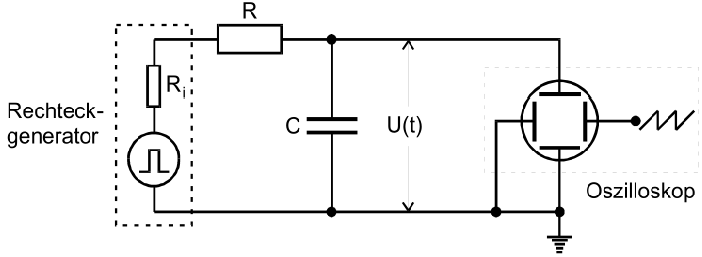
\includegraphics[height=5cm, width=\textwidth]{D1.png}
  \caption{Schaltung zur Messung des Entladevorgangs am Kondensator [1].}
\end{figure}

Bei der zweiten Messreihe wird an dem Generator eine Sinusspannung eingestellt.
Daraufhin wird, wieder mithilfe eines Oszilloskopes, die Amplitude der Spannung am
Kondensator in Abhängigkeit von der am Generator eingestellten Frequenz gemessen.
Für diese Messung wird die in Abbildung 3 gezeigte Schaltung benutzt.

\begin{figure}[H]
  \centering
  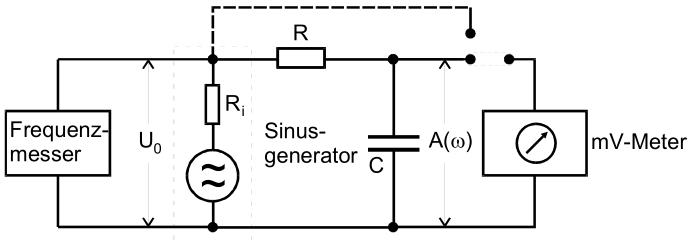
\includegraphics[height=5cm, width=\textwidth]{D2.png}
  \caption{Schaltung zur Messung der Amplitude des Kondensators [1].}
\end{figure}

Nun soll die Phasenverschiebung zwischen der Generatorspannung und der Kondensatorspannung
gemessen werden. Dazu wird ein Zweikanal-Oszilloskop benötigt, wo beide Spannungen
gleichzeitig angezeigt werden. Bei den beiden Spannungen wird zum einen der
zeitliche Abstand der Nulldurchgänge und zum anderen die Periodenlänge der Generatorspannung
in Abhängigkeit von der Frequenz der Generatorspannung gemessen.
In Abbildung 4 sind diese Größen bildlich dargestellt.

\begin{figure}[H]
  \centering
  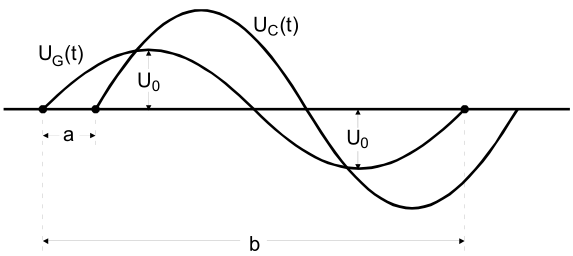
\includegraphics[height=5cm, width=\textwidth]{D4.png}
  \caption{Schaltung zur Messung der Phasenverschiebung [1].}
\end{figure}

\begin{figure}[H]
  \centering
  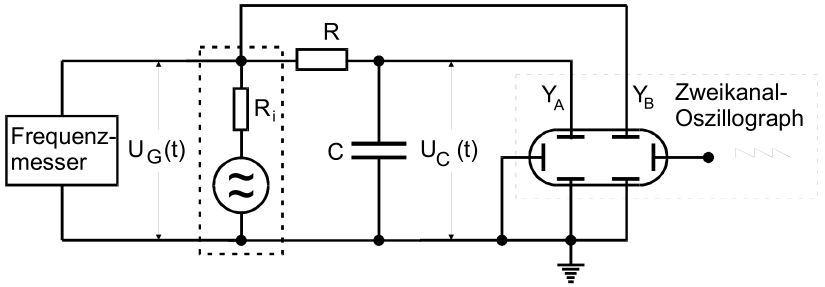
\includegraphics[height=5cm, width=\textwidth]{D3.png}
  \caption{Bildliche Darstellung der Messgrößen [1].}
\end{figure}

Als letztes soll eine Integration dargestellt werden. Dazu wird auch die Schaltung
benutzt, die in Abbildung 5 dargestellt ist. In diesem Fall werden der Reihe nach
Rechteck-, Sinus- und Dreieckspannungen bei dem Generator eingestellt, auf
dem Oszilloskop dargestellt und in Form von Thermodrücken gespeichert.
